\chapter*{Experiment 5 - clap4Led}
\addcontentsline{toc}{chapter}{Experiment 5 - clap4Led}
We wire up the experiment as shown in the diagram fig:~\ref{fig:exp5_microphone}. And upload the sketch code in the next section on page:~\pageref{sketch:exp5}.

%
\begin{figure}[ht]
	\centering
	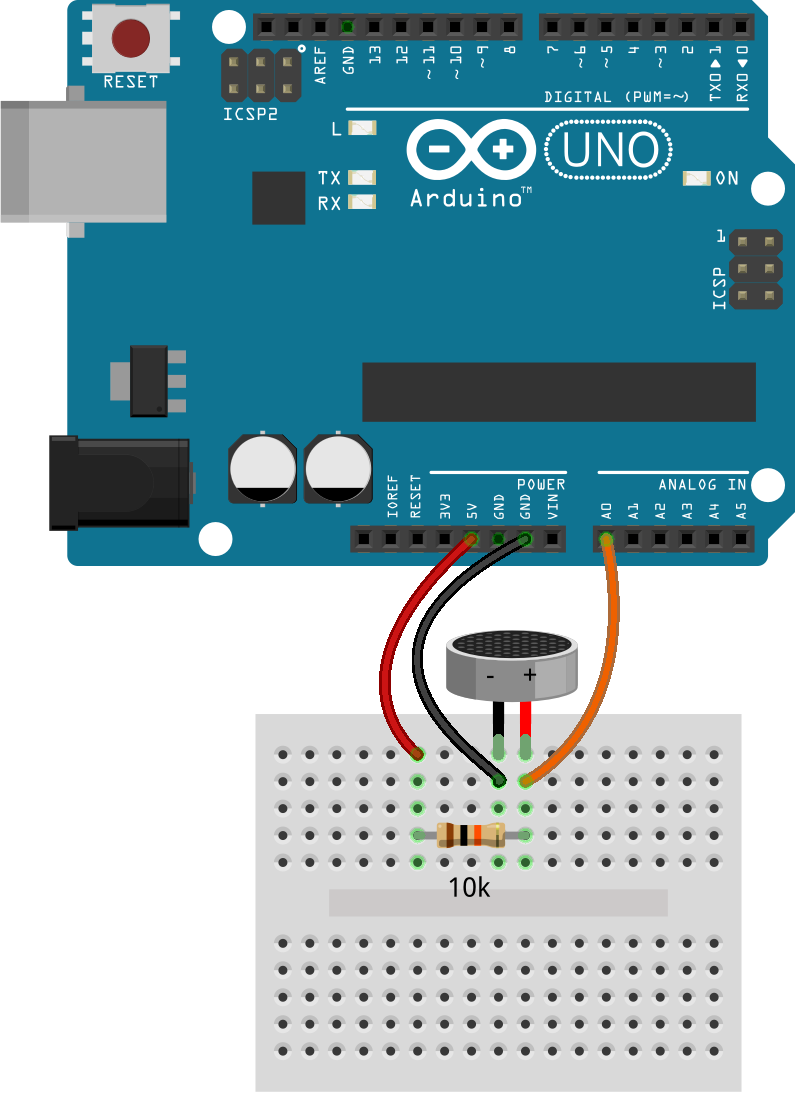
\includegraphics[width=8cm]{images/21}
	\caption{Microphone Activated Circuit}
	\label{fig:exp5_microphone}
\end{figure}
%

The microphone module is polarised, which means it has a positive and negative terminal which must be correctly placed in the circuit in order to function as expected. Please examine the diagram fig:~\ref{fig:exp5_microphone_polarity} on page:~\pageref{fig:exp5_microphone_polarity} to correctly identify which leg is positive and which is negative.

When this circuit is complete, the LED onboard the Arduino will flash when the microphone detects sound.

%
\begin{figure}[ht]
	\centering
	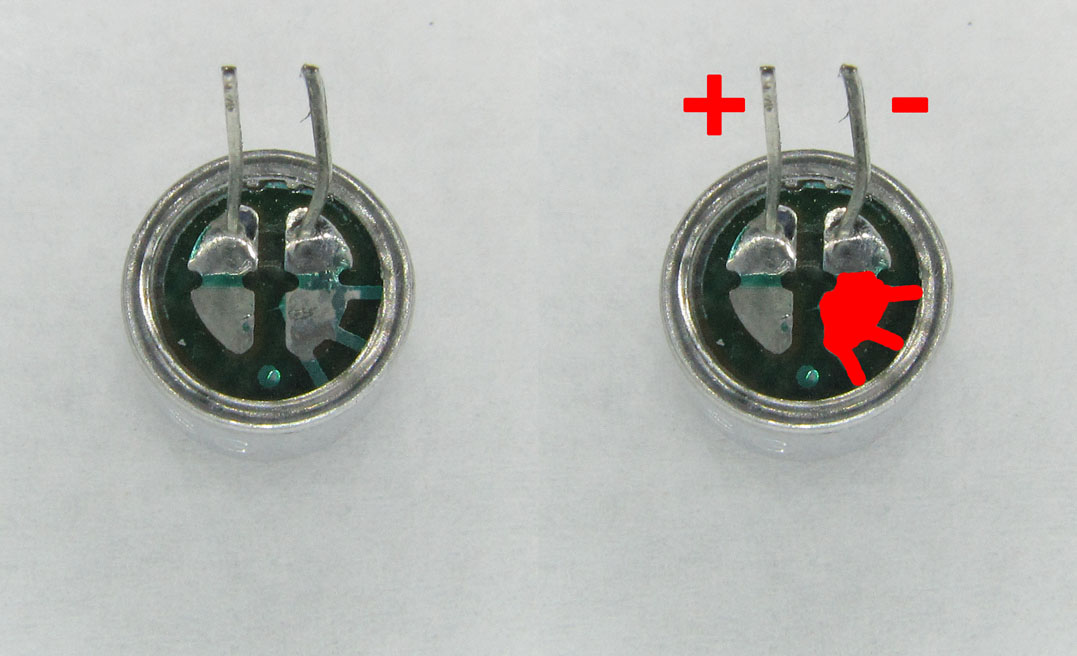
\includegraphics[width=12cm]{images/22}
	\caption{Microphone Module Polarity}
	\label{fig:exp5_microphone_polarity}
\end{figure}
%


\newpage
\section*{Sketch Code}
\label{sketch:exp5}
\begin{lstlisting}
/*
Phenakistoscope
Turns on an LED on then off 20 times a second in order to activate the Phenakistoscope
*/

// the setup function runs once when you press reset or power the board
void setup() {
  // initialize digital pin 13 as an output.
  pinMode(13, OUTPUT);
}

// the loop function runs over and over again forever
void loop() {
  // turn the LED on 
  // (HIGH is the voltage level)
  digitalWrite(13, HIGH);
	
  //wait for 10 milliseconds
  delay(10);
	
  // turn the LED off by making 
  // the voltage LOW
  digitalWrite(13, LOW);    
	            
  // wait for 30 milliseconds              
  delay(30);
}
\end{lstlisting}